\section{Introduction}
\emph{We are given an array that contains N numbers and would like to determine if there are two numbers whose sum equals a given number K.\\
For example we may be given the sequence 4,1,5,2,6,3 and are asked to find a pair of numbers with a sum of 10. In this example 4 and 6 is a valid result.\\
To solve the portfolio do the following:}
\begin{itemize}
\item \emph{Implement an O\(\left( { N }^{ 2 } \right)\) algorithm for solving the problem.}
\item \emph{Implement an O\(\left( N\log {N }  \right) \) algorithm for solving the problem. (Hint: Consider sorting the list.)}
\item \emph{Perform experiments with different values of \textit{N} (generate the associated random lists yourselves)
and plot the time as function of \textit{N}, to verify the time complexity.}
\end{itemize}
\emph{You may use a build in sorting algorithm and assume that it sorts in \(\left( N\log {N }  \right) \).}

\section{Use of algorithms}
\todo[inline]{short introduction}
\subsection{O\(\left( { N }^{ 2 } \right)\)}
\todo[inline]{Description af the algorithm}
\todo[inline]{Pseudocode}
\subsection{O\(\left( N\log {N }  \right) \)}
\todo[inline]{Description af the algorithm}
\todo[inline]{Pseudocode}


\newpage
\section{Verify the time complexity}

\subsection{O\(\left( { N }^{ 2 } \right)\)}
Figure \ref{fig:test1} shows an ideal O\(\left( { N }^{ 2 } \right)\) complexity and the data samples is plotted, time as function of elements. If you compare the plots according to the rate of change the curves are exactly alike. 


\begin{figure}[th!]
\centering
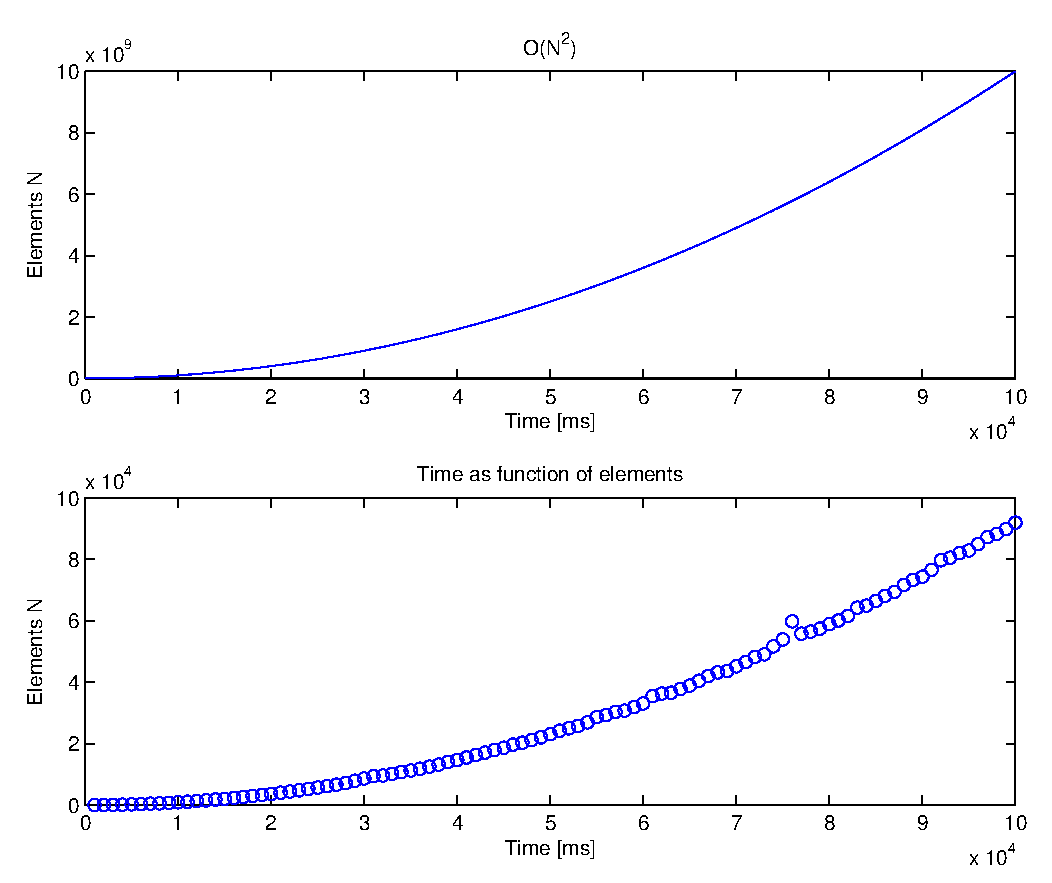
\includegraphics[width=1\textwidth]{./graphics/test1.eps}
\caption{Show plots of an ideal O\(\left( { N }^{ 2 } \right)\) complexity and data samples from the used algorithm.}

\label{fig:test1}
\end{figure}
\newpage


\subsection{O\(\left( N\log {N }  \right) \)}
Figure \ref{fig:test2} shows an ideal O\(\left( N\log {N }  \right) \) complexity and the data samples plotted as time as function of elements. If you compare the plots according to the rate of change the curves they are exactly alike. 



\begin{figure}[th!]
\centering
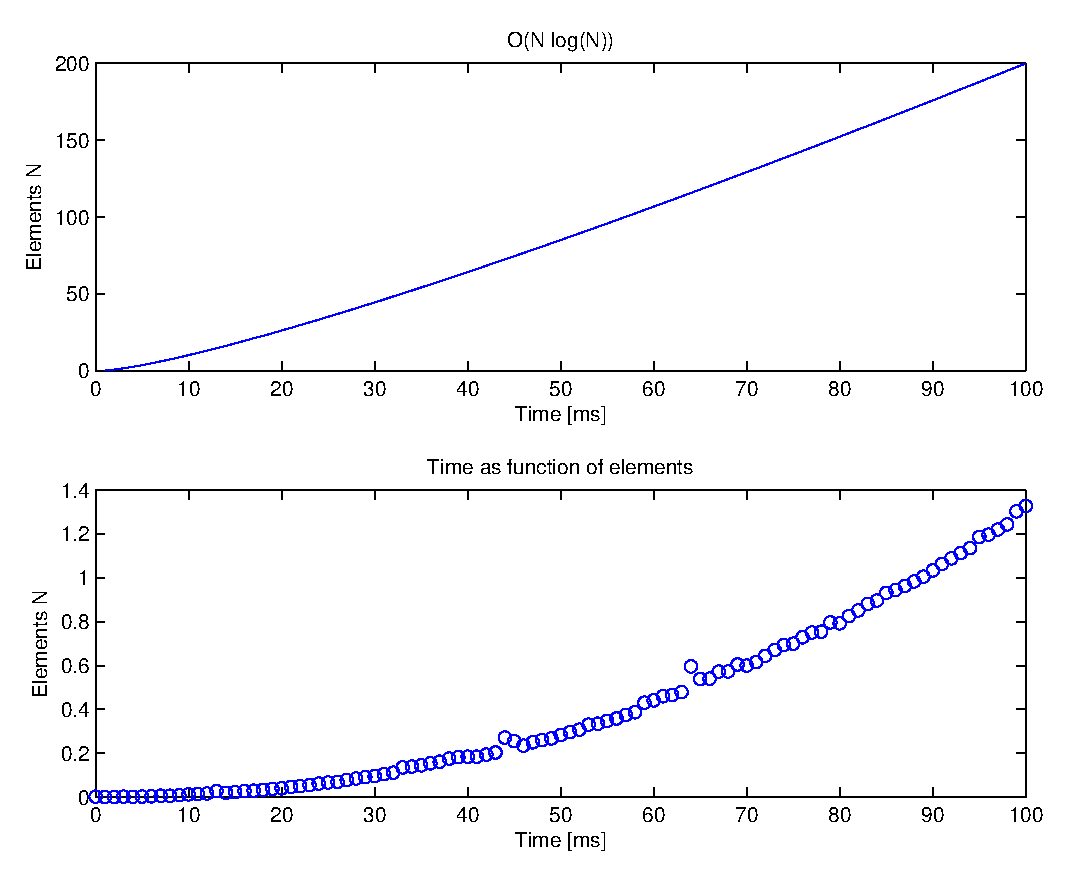
\includegraphics[width=1\textwidth]{./graphics/test2.eps}
\caption{Show plots of an ideal O\(\left( N\log {N }  \right) \) complexity and data samples from the used algorithm.}
\label{fig:test2}
\end{figure}



O\(\left( { N }^{ 2 } \right)\)

O\(\left( N\log {N }  \right) \)